\documentclass{article}
\usepackage{amsmath}
\usepackage{graphicx}
\title{Lösa ekvationssystem numeriskt med gradientmetod???}
\author{Clas Östman}
\date{mars 2023}
\begin{document}
   \maketitle
   Lös ekvationssystemet,
\begin{equation}
    \mathbf{Ax}=\mathbf{b}
\end{equation}
där $\mathbf{A}$ är en känd $n\times n$ matris och $\mathbf{b}$ är en känd $n\times 1$
vektor
Låt $\mathbf{\tilde{x} }$ vara en gissning på lösningen.
Sätt residualen $\mathbf{r}$ till,
\begin{equation}
    \mathbf{r} = \mathbf{A\tilde{x}} - \mathbf{b}
\end{equation}
När $\mathbf{r}$ går mot $\mathbf{0}$ går  $\mathbf{\tilde{x} }$ mot lösningen.
Det är det samma som att beloppet av $\mathbf{r}$ går mot $0$ och därmed att 
$\mathbf{r}^\mathbf{T}\mathbf{r}$
går mot $0$.
Låt $f = \mathbf{r}^\mathbf{T}\mathbf{r}$. 
Gradienten till $f$ i en punkt $\boldsymbol{\xi}$, $\nabla f(\boldsymbol{\xi})$, 
pekar i den riktning där $f$ växer snabbast men det betyder också att
$f$ avtar snabbast i riktningen $- \nabla f(\boldsymbol{\xi})$. Om jag hela tiden går 
steg i den riktning där $f$ avtar snabbast borde jag i sinom tid komma till en punkt 
där $f = 0$ eller åtminstone tillräckligt nära $0$.
\begin{equation}
    \mathbf{r} =  \mathbf{Ax} - \mathbf{b}
\end{equation}
\begin{equation}
    \mathbf{A} = \begin{bmatrix}
        a_{11} & a_{12} & \cdots & a_{1n} \\
        a_{21} & a_{22} & \cdots & a_{2n} \\
        \vdots  & \vdots  & \ddots & \vdots  \\
        a_{n1} & a_{n2} & \cdots & a_{nn} 
    \end{bmatrix}      
\end{equation}
\begin{equation}
    r_i =\sum_{j = 1}^{n}  a_{ij}x_j - b_i
\end{equation}
\begin{multline*}
    f = \mathbf{r}^\mathbf{T}\mathbf{r} = \sum_{i=1}^{n}  r_i^2 = \\
    = (a_{11}x_1 + a_{12}x_2 + \cdots +a_{1n}x_n  - b_1)(a_{11}x_1 + a_{12}x_2 + \cdots
     +a_{1n}x_n  - b_1)+ \\
    + (a_{21}x_1 + a_{22}x_2 + \cdots +a_{2n}x_n  - b_2)(a_{21}x_1 + a_{22}x_2 + \cdots
     +a_{2n}x_n  - b_2)+ \\
     \vdots \\
    + (a_{n1}x_1 + a_{n2}x_2 + \cdots +a_{nn}x_n  - b_n)(a_{n1}x_1 + a_{n2}x_2 + \cdots
     +a_{nn}x_n  - b_n) =
\end{multline*}
\begin{align*}
    = & a_{11}^2 x_1^2 + a_{11}a_{12} x_{1}x_2 + \ldots + a_{11}a_{1n} x_1x_n - 
    a_{11}b_1x_1 +  \\
    + & a_{11}a_{12} x_1x_2 + a_{12}^2 x_2^2 + \ldots + a_{12}a_{1n} x_2x_n - 
    a_{12}b_1x_2 + \\
    + & a_{11}a_{1n} x_1x_n + a_{12}a_{1n} x_2x_n + \ldots + a_{1n}^2 x_n^2 - 
    a_{1n}b_1x_n + \\
    - & a_{11}b_1 x_1 - a_{12}b_1 x_2 - \ldots - a_{1n} b_1 x_n + 
    b_1^2  \\    
     + & \ldots = \\
\end{align*}
\[
    = \sum_{i = 1}^{n} \sum_{j=1}^{n}a_{ij}^2 x_j^2 + 2\sum_{i = 1}^{n} \sum_{j = 1}^{n} 
    \sum_{k=1, k \ne j}^{n} a_{ij}a_{ik} x_j x_k - 2 \sum_{i = 1}^{n} 
    \sum_{j = 1}^{n} a_{ij}b_i x_j + \sum_{i = 1}^{n} b_i^2
\]
\begin{gather*}
    f_{x_i} = \frac{\partial f}{\partial  x_i} = \\
    =2 \sum_{j=1}^{n} a_{ji}^2 x_i + 2 \sum_{j=1}^{n} 
    \sum_{k = 1, k \ne i}^{n}a_{ji}a_{jk} x_k
    - 2 \sum_{j=1}^{n} a_{ji} b_j \\
    = 2 \sum_{j=1}^{n} a_{ji} \left( \sum_{k = 1}^{n} a_{jk} x_k - b_j \right)    
\end{gather*}

Det här är den i:te komponenten i vektorn som, med lämpligt vald koefficient, 
ska dras bort från $\mathbf{x}$. I komponenten kan man se termen,
\[
    \sum_{k = 1}^{n} a_{jk} x_k - b_j
\]
Den är ju lika med $0$ när $\mathbf{x}$ är lösningen. Det betyder att gradienten 
är $\mathbf{0}$ vid lösningen. Det kommer sig av att 
$\mathbf{r}^\mathbf{T}\mathbf{r}>=0$ och därför har minimum 
vid lösningen.
Istället för att beskriva gradienten med den jobbiga summan kan man skriva,
\begin{equation}
    \nabla f = 2 \mathbf{A}^\mathbf{T} (\mathbf{A} \mathbf{x} - \mathbf{b}) =  2 \mathbf{A}^\mathbf{T} \mathbf{r}  
\end{equation}
Nu har jag riktningen jag ska gå i men hur stora kliv ska jag ta?
Jag definierar $\gamma$ som den faktor som multipliceras med den normaliserade
 gradienten för att, förhoppningsvis, komma närmare lösningen.
\begin{equation*}
    \gamma = \frac{(\mathbf{r}^\mathbf{T}\mathbf{r})^{3/2}}{\mathbf{r}^\mathbf{T}\mathbf{A}\mathbf{r}}
\end{equation*}
Då kan jag iterera mig fram till lösningen på följande vis:
\begin{gather*}
    \mathbf{x}_0 = \mathbf{\tilde{x} }
\end{gather*}
Repetera:
\begin{equation*}
    \mathbf{r} = \mathbf{A}\mathbf{x}_i - \mathbf{b}
\end{equation*}

    Beräkna $\gamma $

    Beräkna $\nabla f$
\begin{gather*}
        \mathbf{x}_{i+1} = \mathbf{x}_i - \gamma \frac{\nabla f}{\left\lvert \nabla f\right\rvert } 
\end{gather*}


\newpage
Ett 2-dimensionellt exempel med lösningen, $x_1 = 1, x_2 = 2$.
\begin{equation*}
\left(
    \begin{matrix}
        2 & 1 \\
        1 & 2
    \end{matrix}
    \right) 
\left(
    \begin{matrix}
        x_1 \\
        x_2
    \end{matrix}
\right) = 
\left(
    \begin{matrix}
        4 \\
        5
    \end{matrix}
\right)
\end{equation*}

\begin{figure} 
    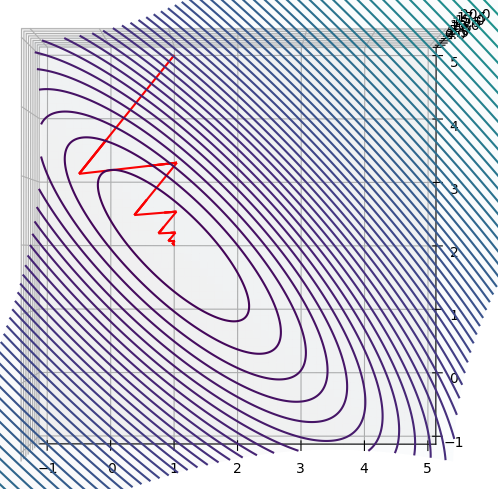
\includegraphics[width=\textwidth]{exempel.png}
  \end{figure}
\newpage  
\begin{verbatim}
    import matplotlib.pyplot as plt
    import numpy as np
    
    # function definition to compute magnitude of a vector
    def magnitude(vector):
        return np.sqrt(sum(pow(element, 2) for 
        element in vector))
    
    def fun(x, y):
        return 5*x**2 + 5*y**2 + 8*x*y - 26*x - 28 *y + 41
    
    # function to calculate the gradient of f
    def grad(a, r):
        return 2*np.matmul(np.transpose(a), r)
    
    # function to calculate the multiplicator gamma
    def gamma(a, r):
        rtr = np.sqrt(np.matmul(np.transpose(r),r))
        return rtr**3/np.matmul(np.transpose(r),np.matmul(a, r))
        
    #Plot setup
    ax = plt.figure().add_subplot(projection='3d')
    # Customize the axis.
    ax.set_xlim(-1, 5)
    ax.set_ylim(-1, 5)
    ax.set_zlim(0, 20)
    # Make data.
    x = np.arange(-1, 5, 0.01)
    y = np.arange(-1, 5, 0.01)
    x, y = np.meshgrid(x, y)
    z = fun(x, y)
    
    # Plot the surface.
    #surf = ax.plot_surface(x, y, z, cmap=cm.coolwarm,
    #                       linewidth=0, antialiased=False)
    surf = ax.plot_surface(x, y, z, alpha = 0.02)
    
    CS = ax.contour(x, y, z, 100)
    ax.clabel(CS, inline=True, fontsize=10)
    
    #Define the arrays
    a = 1.0*np.array([[2, 1],
                      [1, 2]])
    
    b = 1.0*np.array([4, 5])

    
    # initial guess
    x = 1.0*np.array([1, 5])
    
    for i in range(12):
        r = np.matmul(a, x) - b
        gradienten = grad(a, r)
        g = gamma(a, r)*gradienten/magnitude(gradienten)
    
        # draw vectors
        ax.quiver(x[0], x[1], 0, -g[0], -g[1], 0,
                  length=1, color = 'r')
    
        x -= g
        print("x = ", x)
    
    plt.show()
\end{verbatim}
Output:
\begin{verbatim}
x =  [-0.49663635  3.12920456]
x =  [1.04269474 3.30591149]
x =  [0.37358494 2.48134609]
x =  [1.03538137 2.53560304]
x =  [0.75340786 2.19281458]
x =  [1.02054343 2.20571459]
x =  [0.90924198 2.0721461 ]
x =  [1.00984636 2.07354768]
x =  [0.96895199 2.02506783]
x =  [1.00408531 2.02433466]
x =  [0.99018339 2.00804235]
x =  [1.00149442 2.00741015]
\end{verbatim}
\newpage
\begin{figure}
    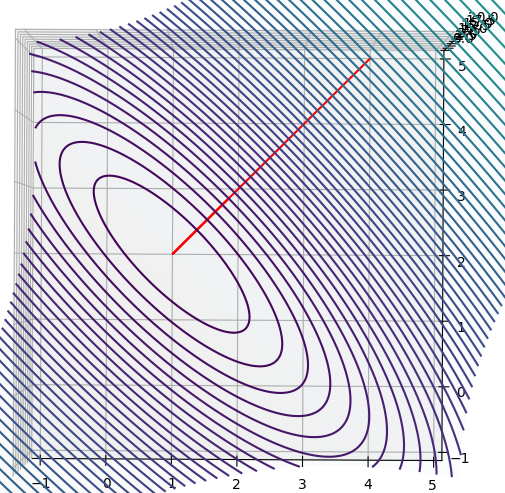
\includegraphics[width=\textwidth]{exempel_2.png}
\end{figure}
Om jag har tur med startgissningen hittas lösningen med bara en iteration!! 
Måste betyda att jag hittat rätt i beräknandet av faktorn $\gamma$.
Tyvärr kan jag inte ta åt mig äran av den uträkningen. Hittade en formel
som jag modifierade lite.

Output:
\begin{verbatim}
x =  [1. 2.]
x =  [1. 2.]
/Users/clasostman/misc/gradeq2d.py:18: RuntimeWarning: invalid 
value encountered in scalar divide
  return rtr**3/np.matmul(np.transpose(r),np.matmul(a, r))
\end{verbatim}
\end{document}
